\documentclass[a4paper, 10pt]{article}
\usepackage[margin=0.5in]{geometry}
\usepackage{comment} % enables the use of multi-line comments (\ifx \fi) 
\usepackage{lipsum} %This package just generates Lorem Ipsum filler text. 
\usepackage{fullpage} % changes the margin
\usepackage{multirow}	
\usepackage{amssymb}
\usepackage{amsmath}
\usepackage{graphicx}
\usepackage{listings}
\usepackage{hyperref}

\newcommand\tab[1][1cm]{\hspace*{#1}}
\newcommand{\psibold}{\pmb{\psi}}
\newcommand{\sumjnminus}{\sum_{j=1}^{n{*}^{-}}}
\newcommand{\kNormal}{k_N(\yi| \thi, \phi)}
\newcommand{\hFn}{h(\thi|\mu,\tausq,\phi, \yi)}
\newcommand{\yi}{y_i}
\newcommand{\Smu}{\sumjn \startheta}
\newcommand{\sumjn}{\sum_{j=1}^{n^*}}
\newcommand{\mfrac}{\frac{\mu \phi +\yi\tausq}{\phi + \tausq} }
\newcommand{\nstar}{n^*}
\newcommand{\startheta}{\theta_j^*}
\newcommand{\thi}{\theta_i}
\newcommand{\thetsq}{\theta^2}
\newcommand{\wbold}{\pmb{w}}
\newcommand{\ybold}{\pmb{y}}
\newcommand{\thetbold}{\pmb{\theta}}
\newcommand{\tausq}{\tau^2}
\newcommand{\aphi}{a_\phi}
\newcommand{\bphi}{b_\phi}
\newcommand{\phiplustau}{\phi+\tausq}
\newcommand{\aalpha}{a_\alpha}
\newcommand{\balpha}{b_\alpha}
\newcommand{\amu}{a_\mu}
\newcommand{\bmu}{b_\mu}
\newcommand{\atau}{a_{\tausq}}
\newcommand{\btau}{b_{\tausq}}
\newcommand{\ind}{\stackrel{ind}{\sim}}
\newcommand{\iid}{\stackrel{iid}{\sim}}
\newcommand{\norm}[1]{\left\lVert#1\right\rVert}
\newcommand{\parenth}[1]{\left(#1\right)}
\newcommand{\bkSquares}[1]{\left[#1\right]}
\newcommand{\curlies}[1]{ \left\{#1\right\} }
\newcommand{\absval}[1]{ \left|#1\right| }
\newcommand{\mat}{ \begin{pmatrix} }
\newcommand{\tam}{ \end{pmatrix} }
\newcommand{\sumi}{ \sum_{i=1}^n }
\newcommand{\prodi}{ \prod_{i=1}^n }
\newcommand{\ds}{ \displaystyle }
\newcommand{\Gpsi}{G_0(\psi)}
\newcommand{\paramSeq}[2]{#1_1,...,#1_{#2}}
\newcommand{\boldpi}{\pmb{\pi}}
\newcommand{\fancyP}{\mathcal{P}}
\newcommand{\thetEJ}[1]{\theta_{e_{j,#1}}}
\newcommand{\elementEJ}[1]{e_{j,#1}}
\begin{document}
%Header-Make sure you update this information!!!!
\noindent
\textbf{STAT 222 Homework \#3} \hfill \textbf{Mary Silva}\\
UCSC \hfill  18 May 2020\\
\\
\begin{enumerate}
    \item[\textbf{1.}] Assume that $\thi | G \iid G$ for $i = 1,...,n$, with $G|\alpha, \psi \sim DP(\alpha, \Gpsi)$, where $\Gpsi$ is a continuous distribution (i.e. it has no atoms) with density $g_0$. Then marginalizing G over its DP prior, the joint distribution for the $\thi$ can be written as 
    $$p(\paramSeq{\theta}{n}|\alpha,\psi) = \sum_{\boldpi \in \fancyP} p (\boldpi|\alpha) \curlies{\prod_{j=1}^{n^*} g_0(\thetEJ{1}| \psi) \prod_{i=2}^{n_j} \delta_{\thetEJ{1}}(\thetEJ{i}) } $$
    where $\fancyP_n$ denotes the set of all partitions $\boldpi = \curlies{s_j:j=1,...,n*}$ of $\curlies{1,...,n}$ and $p(\boldpi|\alpha)$  the DP-implied prior probability for partition $\boldpi$. Here $n^*$ is the number of cells of that partition $\boldpi$, $n_j$ is the number of elements in cell $s_j$, and $\elementEJ{1} < ... < \elementEJ{n_j}$ are the elements of cell $s_j$. \\\\
    Let $\nstar(n) = \sum_{i=1}^{n} U_i$, where $U_i$ is a binary random variable indicating whether $\thi$ is a new value drawn from $G_0$ or not. We show by induction that 
    $$p(\boldpi|\alpha) = \frac{\alpha^{n^*}}{\alpha^{(n)}} \prod_{j=1}^{n^*} (n_j - 1)!$$
    
    For the base case $n=0$, this is obviously true. We assume, then that it holds for all $n=k$. 
    By the induction hypothesis we have 
    \begin{align*}
    p(\paramSeq{\theta}{k}|\alpha,\psi) = \sum_{\boldpi\in\fancyP} \frac{\alpha^\nstar}{\Gamma(\alpha+k) \Gamma(\alpha)} \prod_{j=1}^{\nstar} (n_j -1)! \curlies{\prod_{j=1}^{n^*} g_0(\thetEJ{1}| \psi) \prod_{i=2}^{n_j} \delta_{\thetEJ{1}}(\thetEJ{i}) }
    \end{align*}
    By exchangeability, the probability depends on the sizes of the partitioning sets. The probability that partitioning set of size $n_1$ consists of the first $n_1$ variables, $n_2$ of the next $n_2$ variables, and so on, can be obtained can be obtained by multiplying the probabilities for consecutive draws in the P`olya urn scheme. Let 
    
    For 
    \begin{align*}
        p(\curlies{s_1,...,s_{k+1}}| \alpha) &= \frac{\alpha}{\alpha}\frac{1}{\alpha+1} \ldots 
        \frac{n_1 -1}{\alpha + n_1 -1} \times \ldots \times 
        \frac{\alpha}{\alpha + \sum_{j = 1}^k n_j} \frac{1}{\alpha + \sum_{j = 1}^k n_j + 1} \ldots 
        \frac{n_{k-1}-1}{\alpha + \sum_{k=1}^{k} n_j + n_{k-1} -1 }\\
        & = \displaystyle\frac{\alpha^{\nstar(k+1)}}{\Gamma(\alpha + k + 1) \Gamma(\alpha)} \prod_{j=1}^{\nstar(k+1)} (n_j - 1)!
    \end{align*}
    Thus, by induction, the proof holds. I obviously didn't spend too much time on this problem. Problem 2 took a lot out of me.
    
    \item[\textbf{2.}] Consider the location normal DP mixture model:
    \begin{align*}
        &f(y|G,\phi) = \int k_N(y|\theta,\phi) dG(\theta), &G|\alpha,\mu,\tausq \sim DP(\alpha, G_0 = N(\mu, \tausq))     
    \end{align*}
    Where $k_N(\cdot|\theta,\phi)$ denotes the density function of the normal distribution with mean $\theta$ and variance $\phi$. We assume an $IG(a_\phi, b_\phi)$ prior for $\phi$, and $Gamma(\aalpha, \balpha)$ prior for $\alpha$, and take $N(\amu, \bmu)$ and $IG(\atau, \btau)$ priors for the mean and variance, $\mu$ and $\tausq$, respectively, for the centering distribution $G_0$. Therefore, the hierarchical version of this semiparametric DP mixture model is given by
    
    \begin{align*}
        \yi|\thi, \phi &\ind N(\yi|\thi, \phi), i = 1,...,n\\
        \thi|G &\iid G, i = 1,...,n\\
        G|\alpha,\mu,\tausq &\sim DP(\alpha, G_0 = N(\mu, \tausq))\\
        \alpha, \mu,\tausq,\phi &\sim p(\alpha)p(\mu)p(\tausq)p(\phi)
    \end{align*}
    with the independent priors $p(\alpha), p(\mu), p(\tausq),$ and $p(\phi)$ for $\alpha, \mu, \tausq, \phi$ given above.
    
    \begin{enumerate}
        \item[(2.1)] \textbf{Expressions for the full conditionals.} We derive the expressions for the full conditionals of the P\`olya urn based Gibbs sampler, which can be used for posterior simulation from $p(\thetbold, \alpha, \phi, \mu, \tausq|data)$, where $data=\curlies{\yi:i=1,...,n}$.
        
        A key property for the implementation of the Gibbs sampler is the discreteness of G, which includes a partitioning of the $\thi$. From the lecture notes we use the following notation
        \begin{itemize}
            \item $\nstar$: the number of distinct elements(clusters) in the vector $(\theta_1,...,\theta_n)$.
            \item $\startheta, j=1,...,\nstar$: the distinct $\thi$
            \item $\pmb{w} = (w_1,...,w_n)$ is the vector of configuration indicators, defined by $w_i =j$ if and only if $\thi = \startheta, i = 1,...,n$
            \item $n_j$ is the size of the $j^{\text{th}}$ cluster, i.e. $n_j = \absval{\{i: w_i =j \}}, j = 1,...,\nstar$.
        \end{itemize}
        The vectors $\parenth{\nstar, \wbold, \theta_1^*,...,\theta_{\nstar}^* }$ and $(\theta_1, ..., \theta_n)$ are equivalent. \\ 
        
        For each $i = 1,...,n$, $p(\thi|\{\theta_{i'}:i'\ne i\},\alpha,\mu, \tausq, \phi, \ybold)$ is simply a mixture of $n^{*-}$ point masses and the posterior for $\thi$ based on $\yi$,
        \begin{align*}
            \frac{\alpha q_0}{\alpha q_0 + \sumjnminus n_j^{-} q_j } \hFn + \sumjnminus \frac{ n_j^{-} q_j }{ \alpha q_0 + \sumjnminus n_j^{-} q_j} \delta_{\startheta}(\thi)\\
        \end{align*}
        For the purposes of coding, let $A = \frac{\alpha q_0}{\alpha q_0 + \sumjnminus n_j^{-} q_j }$ and $B_j = \frac{ n_j^{-} q_j }{ \alpha q_0 + \sumjnminus n_j^{-} q_j}$, and
        \begin{itemize}
            \item $q_j = k_N(\yi|\startheta, \phi)$
            \item $q_0 = \int \kNormal g_0(\theta| \mu, \tausq) d\theta$
            \item $ \hFn \propto \kNormal g_0(\thi|\mu,\tausq)$
            \item $g_0$ is the density of $G_0 = N(\cdot|\mu,\tausq)$
            \item The superscript ``-'' denotes all relevant quantities when $\thi$ is removed from the vector $\pmb{\theta}$, e.g. $n*^{-}$ is the number of clusters in $\left\{\theta_{i'}: i' \ne i \right\}$
        \end{itemize}
        
        Integrating out $\theta$, we get the following
        \begin{align*}
            q_0  &= \int \kNormal g_0(\theta|\mu, \tausq) d\theta \\
                &= \int \parenth{2\pi \phi}^{-1/2} \exp \curlies{-\frac{1}{2\phi} (\yi -\theta)^2 }\parenth{2\pi\tausq}^{-1/2} \exp \curlies{- \frac{1}{2\tausq} (\theta - \mu)^2} d\theta\\
                &= \parenth{4\pi^2\phi\tausq}^{-1/2} \int \exp \curlies{ - \frac{1}{2\tausq} (\theta - \mu)^2 - \frac{1}{2\tausq} (\theta - \mu)^2 } d\theta\\
                &= \parenth{4\pi^2\phi\tausq}^{-1/2} \int \exp \curlies{ -\frac{1}{2\phi\tausq} \bkSquares{ \tausq \yi - 2\yi \tausq \theta + \tausq\theta^2 + \phi\mu^2 - 2\mu\phi\theta + \phi\theta^2 } } d\theta\\
                &= \parenth{4\pi^2\phi\tausq}^{-1/2} \int \exp \curlies{ \frac{1}{2\phi\tausq} \bkSquares{ \thetsq(\phi + \tausq) - 2\theta(\mu\phi + \yi\tausq ) } - \frac{\phi\mu^2 + \tausq \yi^2}{2\phi\tausq} }d\theta\\
                &= \parenth{4\pi^2\phi\tausq}^{-1/2} \exp \curlies{- \frac{\phi \mu^2 +\tausq \yi^2}{2\phi\tausq} }\\
                &\tab\times\int \exp \curlies{- \frac{\phi + \tausq}{ 2 \phi \tausq  }\bkSquares{\thetsq - 2\theta \parenth{\mfrac } + \parenth{\mfrac}^2 -  \parenth{\mfrac}^2 } }d\theta\\
                &=\parenth{2\pi\phi\tausq}^{-1/2}\parenth{\frac{\phi \tausq}{\phi + \tausq}}^{1/2}\exp \curlies{- \frac{\phi\mu^2 + \tausq \yi}{2\phi\tausq} + 
                            \frac{ \parenth{\mu\phi + \yi\tausq}^2 }{2\phi\tausq(\phi +\tausq)} }\\
                &= \parenth{2\pi(\phi+\tausq)}^{-1/2} \exp \curlies{ \frac{(\phi\mu^2 + \tausq \yi^2)(\phiplustau) + (\mu\phi + \yi\tausq)^2}{2\phi \tausq(\phiplustau) } }\\
                &= \parenth{2\pi(\phi+\tausq)}^{-1/2} \exp \curlies{ \frac{-\phi\mu\tausq - \phi\yi\tausq + 2\mu\phi\tausq}{2\phi \tausq(\phiplustau)}}\\
                &=\parenth{2\pi(\phi+\tausq)}^{-1/2} \exp \curlies{ - \frac{\yi^2 - 2\yi \mu + \mu^2}{2(\phiplustau)}}\\
                &= N(\yi|\mu,\phiplustau)
        \end{align*}
        After dropping all the non $\thi$ terms, we are left with the part that was inside the integral, which is just $h(\thi|\cdot)$, which has a normal distribution with mean $\frac{(\mu\phi+ \yi\tausq)}{\phiplustau}$, and variance $\frac{\phi\tausq}{\phiplustau}$. This completes the marginal posterior for $\thi$.

        We derive the full conditionals for $\mu, \tausq$, and $\phi$:
        \begin{align*}
            p(\mu|\cdot) &\propto \exp \curlies{- \frac{1}{2\bmu}(\mu - \amu )^2} \exp \curlies{- \frac{1}{2\tausq} \sumjn (\startheta - \mu)^2}\\
                &\propto \exp \curlies{-\frac{1}{2\bmu}(\mu^2 - 2\amu\mu + \amu^2) - \frac{1}{2\tausq} \parenth{\sumjn {\startheta}^2 - 2\mu \sumjn \startheta + \nstar\mu^2 }}\\
                &\propto \exp \curlies{-\frac{1}{2\bmu} (\mu^2 - 2\amu \mu) -  \frac{1}{2\tausq} \parenth{ -2 \mu\Smu +\nstar\mu^2 } }\\
                &\propto \exp \curlies{ -\frac{1}{2\bmu \tausq} \parenth{\mu^2\tausq - 2\amu\mu\tausq - 2\mu \Smu \bmu +\mu^2\nstar \bmu } }\\
                &\propto \exp \curlies{ -\frac{1}{2\bmu \tausq} \parenth{\mu^2(\tausq +\bmu \nstar)} -2\mu\parenth{\amu\tausq +\bmu\Smu} } \\
                &\propto \exp \curlies{ - \frac{\tausq +\bmu\nstar}{2\bmu\tausq} \bkSquares{\mu^2 - 2\mu \parenth{\frac{\amu \tausq +\bmu\Smu }{\tausq +\bmu\nstar} } } }
        \end{align*}
        \begin{align*}
            p(\tausq|\cdot) &\propto (\tausq)^{\atau - 1} \exp \curlies{-\frac{\btau}{\tausq}} (\tausq)^{\nstar /2} \exp \curlies{- \frac{1}{2\tausq} \sumjn (\startheta - \mu)^2}\\
                &=(\tausq)^{-(\atau + \nstar/2) - 1} \exp\curlies{-\frac{1}{\tausq}\parenth{\btau + \frac{1}{2}\sumjn (\startheta - \mu)^2}}
        \end{align*}
        
        \begin{align*}
            p(\phi|\cdot) &\propto p(\phi) \prod_{i=1}^{n} k_N(\yi|\thi,\phi)\\
                &\propto \phi^{-\aphi - 1}\exp \curlies{- \frac{\bphi}{\phi}}\prod_{i=1}^n \phi^{-1/2} \exp \curlies{-\frac{1}{2\phi}(\yi-\thi)^2}\\
                &\propto \phi^{-(\aphi + \frac{n}{2})-1} \exp \curlies{-\frac{1}{\phi}\parenth{\bphi + \frac{1}{2} \sum_{i=1}^n (\yi - \thi)^2 } }
        \end{align*}
        Thus, after rearranging the terms, the full conditionals for $\mu$, $\tausq$, and $\phi$ reduce to
        \begin{align*}
            \mu|\cdot &\sim N\parenth{\parenth{\frac{1}{\bmu} + \frac{\nstar}{\tausq} }^{-1} \parenth{ \frac{\amu}{\bmu} + \frac{1}{\tausq} \sum_{j=1}^{\nstar} \startheta }, \parenth{\frac{1}{\bmu} + \frac{\nstar}{\tausq} }^{-1} }\\
            \tausq|\cdot &\sim IG \parenth{\atau + \frac{\nstar}{2}, \btau + \frac{1}{2}\sum_{j=1}^{\nstar} (\startheta - \mu)^2 }\\
            \phi|\cdot &\sim IG\parenth{\aphi + \frac{n}{2}, \bphi + \frac{1}{2} \sum_{i=1}^n (\yi -\thi)^2}
        \end{align*}
        
        The full conditional for $\alpha$ is not standard form. To estimate, we use the exchangeable product partition function (Antoniak, 1974)
        \begin{align*}
            p(\nstar|\alpha) &\propto \alpha^{\nstar} \frac{\Gamma(\alpha)}{\Gamma(\alpha + n )} \\
                &= \frac{\alpha^{\nstar} (\alpha + n)}{\alpha \Gamma(n)} \int_0^1 \eta^\alpha (1-\eta)^{n-1} d\eta
        \end{align*}
        Therefore, we devise a sampler for $\alpha$ by first introducing latent variable $\eta$ such that 
        $$\eta|\alpha,\nstar, \ybold \sim Beta(\alpha + 1, n) $$
        
        Then $\alpha| \eta, \nstar \sim \varepsilon Gamma \parenth{\aalpha + \nstar, \balpha - \log\eta } + (1-\varepsilon) Gamma \parenth{\aalpha + \nstar -1, \balpha - \log \eta }$, where 
        $$\varepsilon = \frac{\aalpha+ \nstar - 1 }{n(\balpha - \log \eta ) + \aalpha + \nstar -1 } $$
    

        This clever auxiliary variable sampler was first introduced in Escobar and West (1995).    
    
        \item[(2.2)] \textbf{Prior specification.} We examine several choices for the hyperparameters for $\phi, \tausq$ and $\mu$. To do this, I chose hyperparameters in such a way that the prior means for each $\phi, \tausq$ and $\mu$ ranged from small to large and observed how the posterior means for $\phi, \tausq$ and $\mu$ changed. 
        \clearpage
        For instance, in Figure \ref{change_mus}, I kept the priors for $\tausq$ and $\phi$ the same while changing the hyperparameters for $\mu$. The posterior mean for $\mu$ didn't change much from the prior mean. As the prior mean for $\mu$ increased, the posterior mean for $\tausq$ changed drastically from the prior mean for $\tausq$. The posterior density for $\phi$ becomes bimodal when the prior mean and prior variance for $\mu$ equals 10 and 3, respectively.
        
        \begin{figure}[h!]
            \centering
            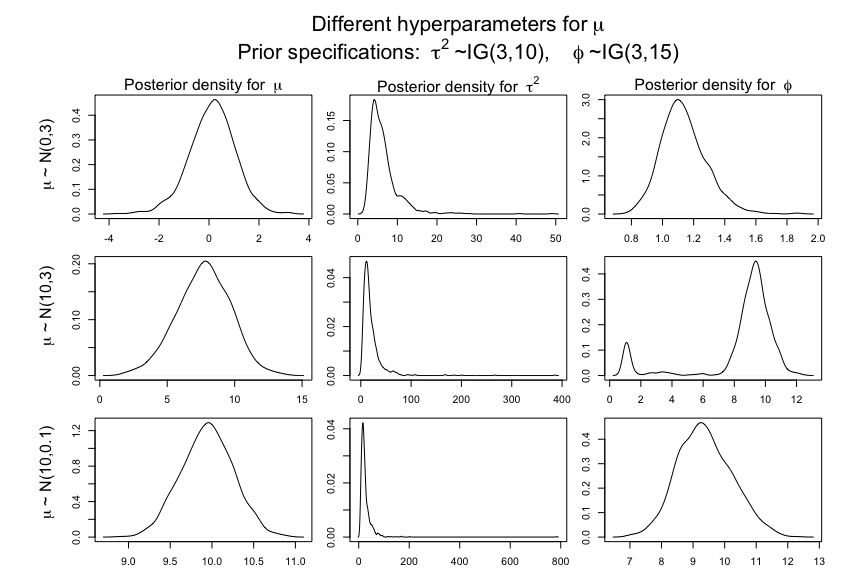
\includegraphics[scale =0.4]{Change_mus.png}
            \caption{Density plots for the posterior samples of $\mu, \tausq$ amd $\phi$ using different choices of hyperparameters for $\mu$.}
            \label{change_mus}
        \end{figure}
        I repeated the process for Figure  \ref{change_taus}. In this case, the posterior means for $\mu$ don't change much. The posterior means for $\tausq$ matches the prior mean for $\tausq$. 
        \begin{figure}[h!]
            \centering
            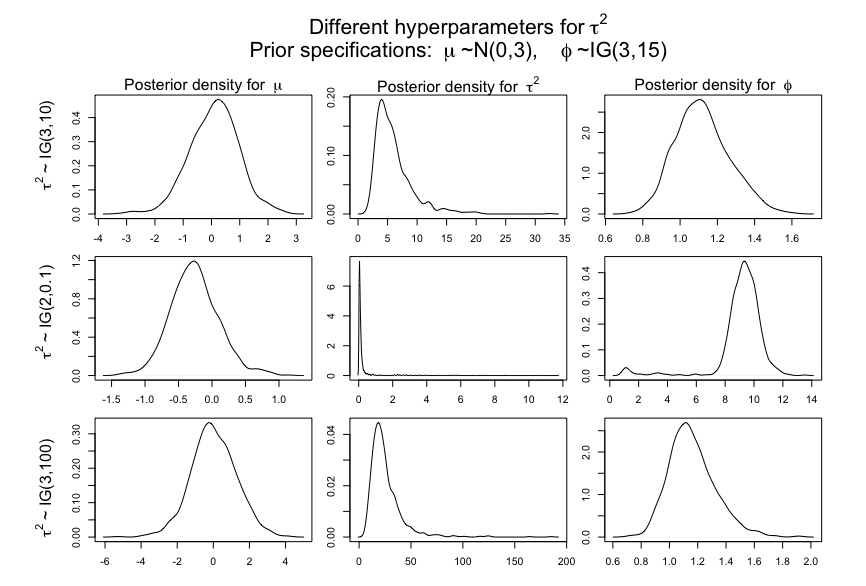
\includegraphics[scale =0.4]{Change_taus.png}
            \caption{Density plots for the posterior samples of $\mu, \tausq$ amd $\phi$ using different choices of hyperparameters for $\tausq$.}
            \label{change_taus}
        \end{figure}
    
        \begin{figure}[h!]
            \centering
            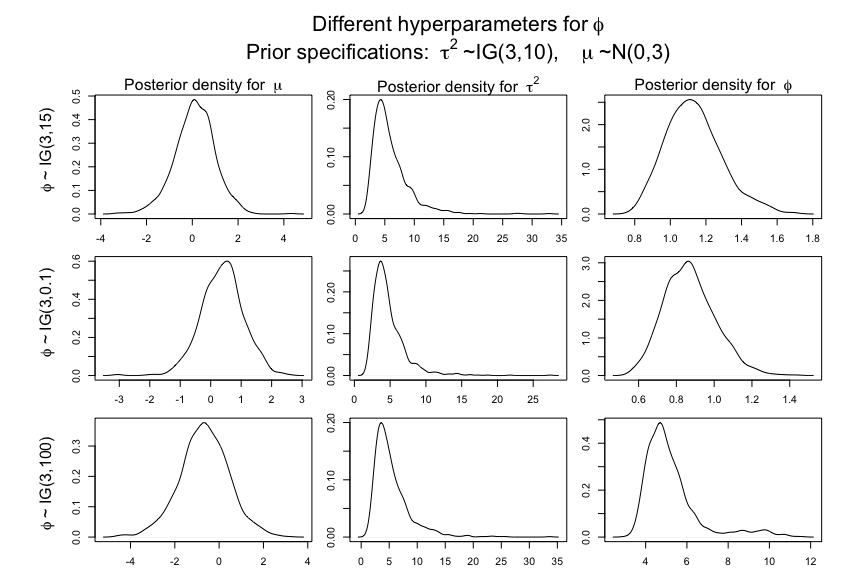
\includegraphics[scale =0.45]{Change_phis.png}
            \caption{Density plots for the posterior samples of $\mu, \tausq$ amd $\phi$ using different choices of hyperparameters for $\phi$.}
            \label{change_phis}
        \end{figure}
    
    After examining the posterior predictive density (see 2.5), I decide ultimately to use the following prior specifications
    \begin{align*}
        \phi &\sim IG(3,15)\\
        \tausq &\sim IG(3,10)\\
        \mu &\sim N(0,3)
    \end{align*}
    \item[(2.3)] \textbf{Prior specifications for} $\pmb{\alpha}$. I chose two prior specifications for $\alpha$ to get an idea how it affects $\nstar$ and posterior predictive inference. I use $\alpha \sim Gamma(1,1)$ and $\alpha \sim Gamma(2,.1)$. Based on figure \ref{nstar}, $\nstar$ is clearly affected by the choice of $\alpha$. For $\alpha \sim Gamma(1,1)$, $\nstar$ ranges from 5 to 9 and for $\alpha \sim Gamma(2,0.1)$, $\nstar$ ranges from 8 to 29.
    \begin{figure}[h!]
        \centering
        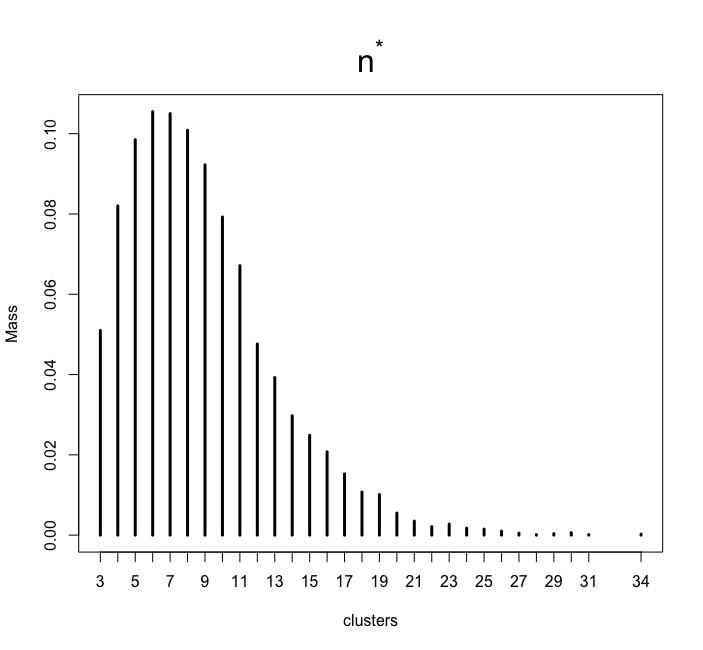
\includegraphics[scale = 0.25]{alpha_n1.png}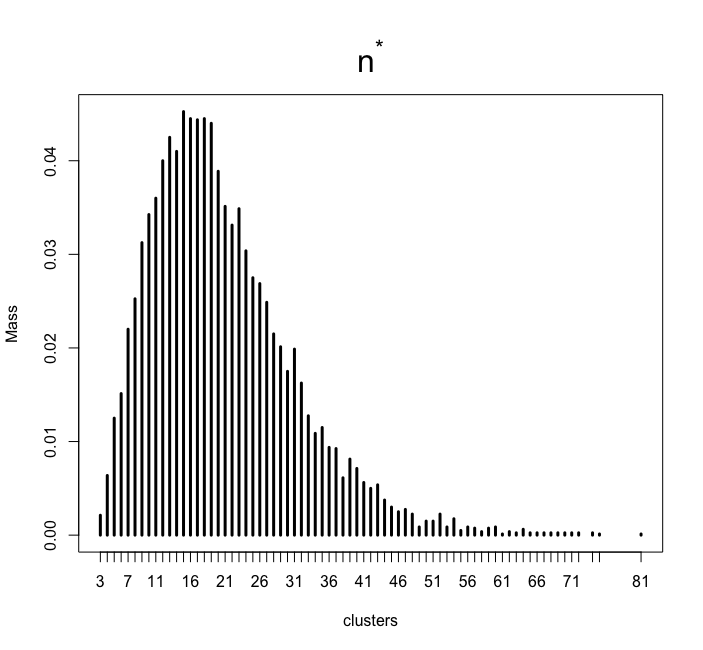
\includegraphics[scale = 0.25]{alpha_n2.png}
        \caption{(Left) Posterior for $\nstar$ with prior $\alpha \sim Gamma(1,1)$. (Right) Posterior for $\nstar$ with prior $\alpha \sim Gamma(2,0.1)$.}
        \label{nstar}
    \end{figure}
    
      \begin{figure}[h!]
        \centering
        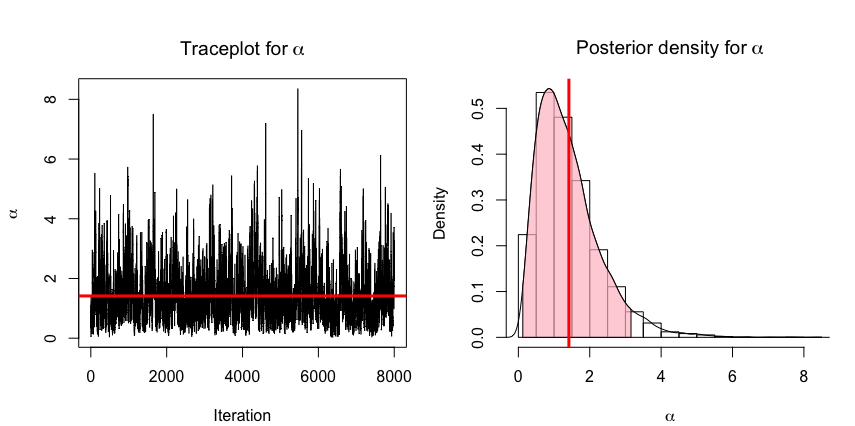
\includegraphics[scale=0.5]{alpha1.png}
        \caption{The traceplot and histogram for the posterior samples of $\alpha$ corresponding to a prior specified by $\alpha \sim Gamma(1,1)$. The pink shaded region represents the 95\% posterior credible interval for the parameter and the solid red line represents the posterior mean.}
        \label{alpha1}
    \end{figure}
    
    \begin{figure}[h!]
        \centering
        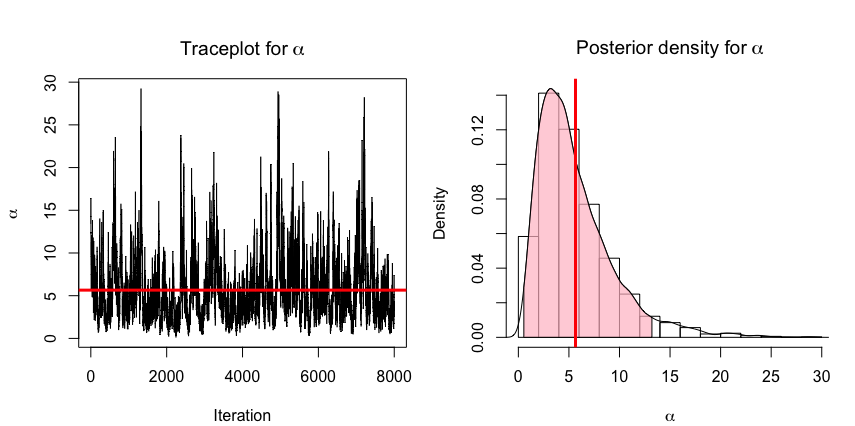
\includegraphics[scale=0.5]{alpha2.png}
        \caption{The traceplot and histogram for the posterior samples of $\alpha$ corresponding to a prior specified by $\alpha \sim Gamma(2,0.1)$. The pink shaded region represents the 95\% posterior credible interval for the parameter and the solid red line represents the posterior mean.}
        \label{alpha1}
    \end{figure}
    Based on figures \ref{nstar} - \ref{alpha1}, $\alpha$ and $\nstar$ are highly sensitive to the prior on $\alpha$.
    \clearpage
    \item[(2.4)] \textbf{Clustering induced by the DP.} Figure \ref{prob2-4} shows each cluster label $\theta_i$, sorted by the order of the observations. 
    
    \begin{figure}[h!]
        \centering
        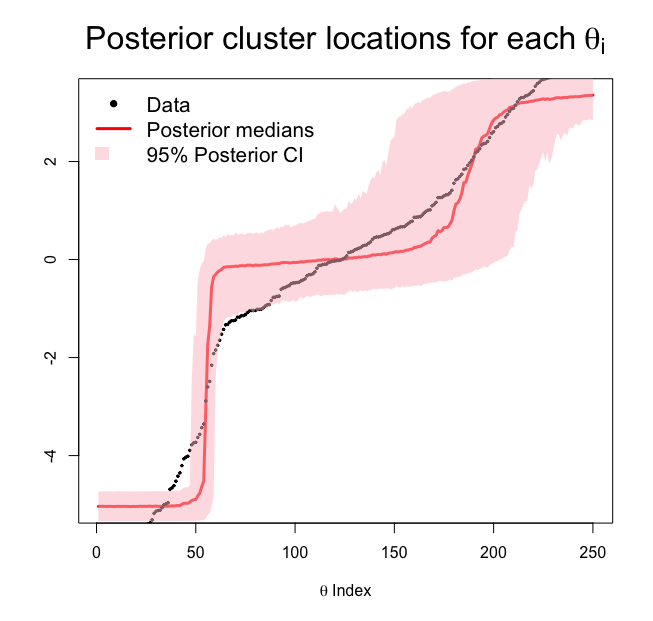
\includegraphics[scale = 0.4]{Posterior_th_clusters.png}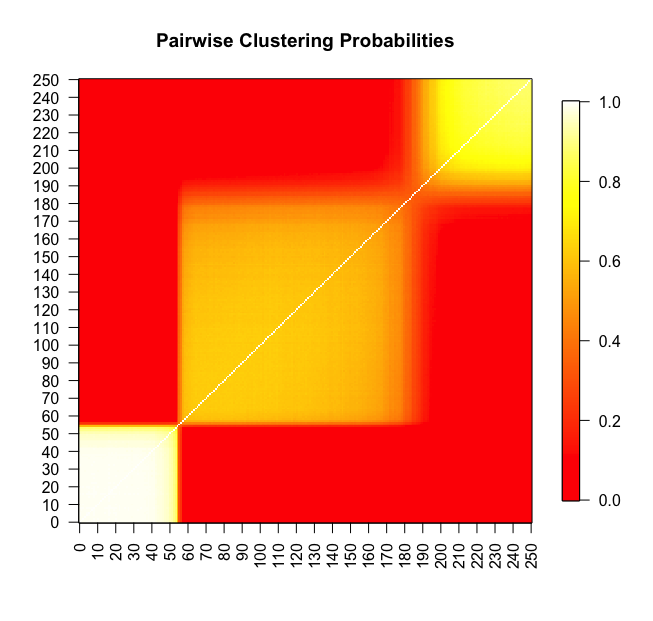
\includegraphics[scale = 0.4]{ClustMatrix.png}
        \caption{Posterior cluster locations for each $\theta_i$ sorted by the order of the magnitude of y.}
        \label{prob2-4}
    \end{figure}
    
    \begin{figure}[h!]
        \centering
        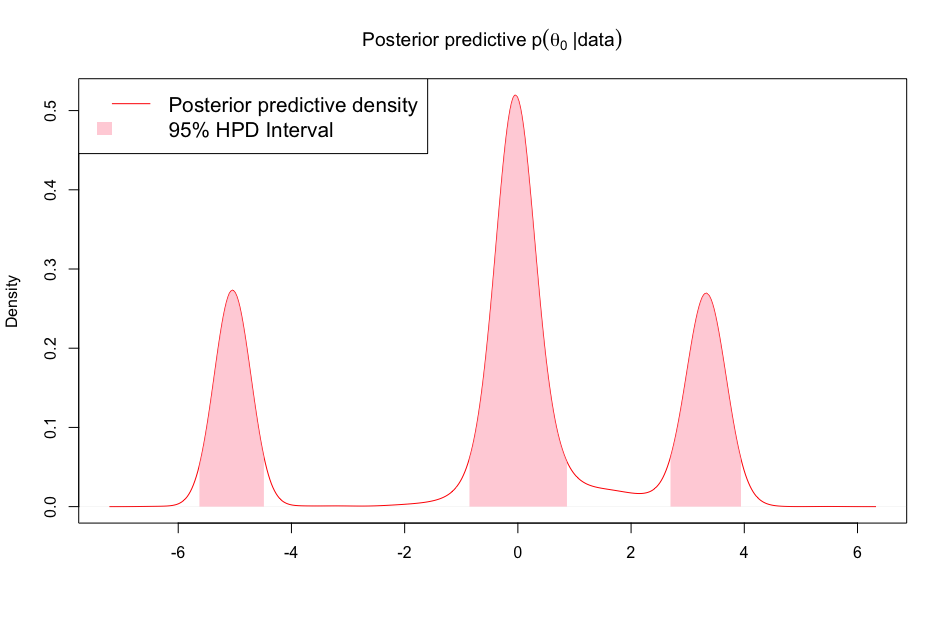
\includegraphics[scale = 0.4]{pptheta.png}
        \caption{(Left) Posterior predictive for $\theta_0$ with corresponding 95\% highest posterior density interval. (Right) From the plot of the pairwise clustering probabilities, we see three distinct groups.}
        \label{pptheta}
    \end{figure}
    
    Based on the above figures \ref{prob2-4} - \ref{pptheta}, there appears to be three clusters for $\theta$'s with medians at -5, 0, and 3. This is also consistent with the true model (i.e. The synthetic data generated from the mixture $0.2N(-5,1) + 0.5N(0,1) + 0.3N(3.5,1)$).
    \clearpage
    \item[(2.5)] \textbf{Posterior predictive density} $\pmb{p(y_0|data)}$. Lastly, we obtain the posterior predictive density and use it to show that the prior specifications capture the distributional shape suggested by the data. Based on figure \ref{ppy}, the model was able to capture the underlying distribution of the data.
    \begin{figure}[h!]
        \centering
        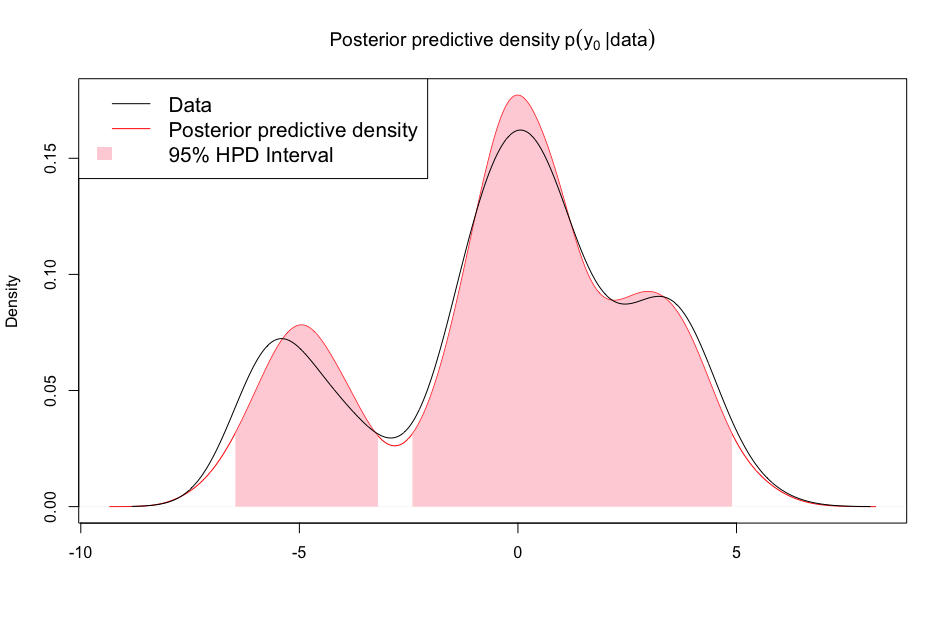
\includegraphics[scale = 0.4]{ppy.png}
        \caption{The posterior predictive for a new data point $y_0$, with corresponding highest posterior density interval shaded in pink.}
        \label{ppy}
    \end{figure}
    \end{enumerate}
    \item[\textbf{3.}] Since this problem was made optional, I am just throwing together plots resulting from the following location-scale normal DP mixture model, which are on the next few pages. This was an attempt to use 
    \begin{align*}
        f(y|G) &= \int k_N(y|\theta, \phi)dG(\theta,\phi), & G|\alpha,\psi &\sim DP(\alpha,G_0(\psibold)),
    \end{align*}
    with the conjugate normal/inverse-gamma specification for the centering distribution
    $$G_0(\theta,\phi|\psibold) = N(\theta|\mu,\phi/\kappa) \times IG(\phi|c,\beta)$$
    for fixed $c$ and random $\psibold = (\mu,\kappa,\beta)$
    
    I specify the model with the following: $c=3$, $\mu\sim N(0, \sqrt{2}^2)$, $\kappa \sim Gamma(1,1)$ and $\beta\sim IG(5,0)$
    \begin{figure}[h!]
        \centering
        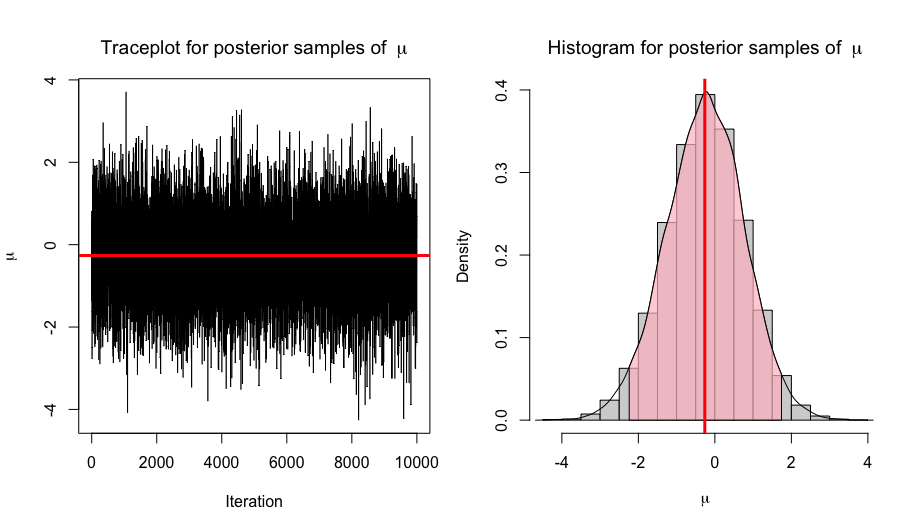
\includegraphics[scale = 0.4]{Prob3_mu.png}\\
        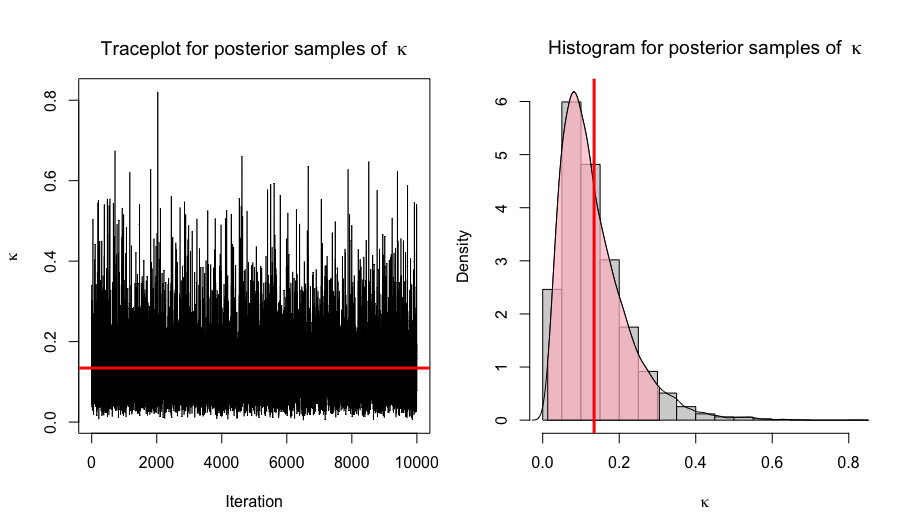
\includegraphics[scale = 0.4]{Prob3_Kappa.png}\\
        % 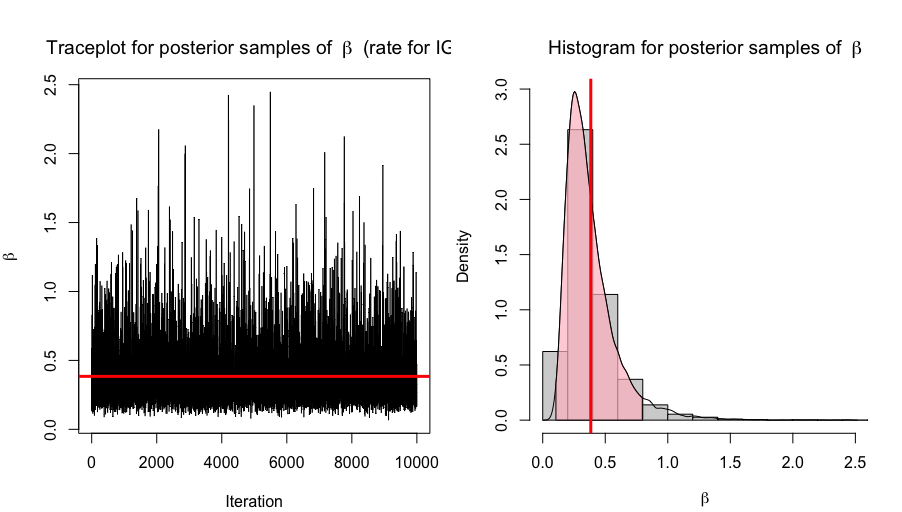
\includegraphics[scale = 0.4]{Prob3_beta.png}\\
        % 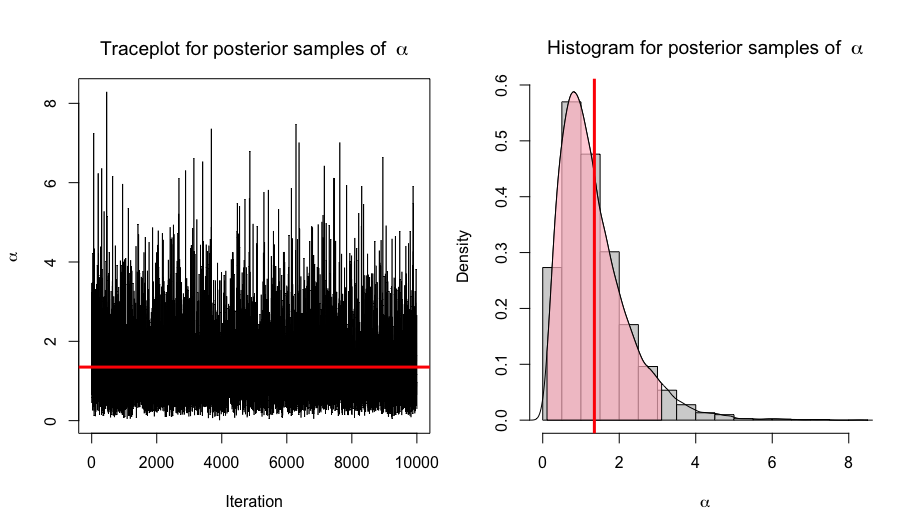
\includegraphics[scale = 0.4]{Prob3_alpha.png}\\
        \caption{Traceplot and histogram for the posterior samples of $\mu$ (top), and $\kappa$ (bottom).}
        \label{prob3_fig}
    \end{figure}
    
    \begin{figure}[h!]
        \centering
        % 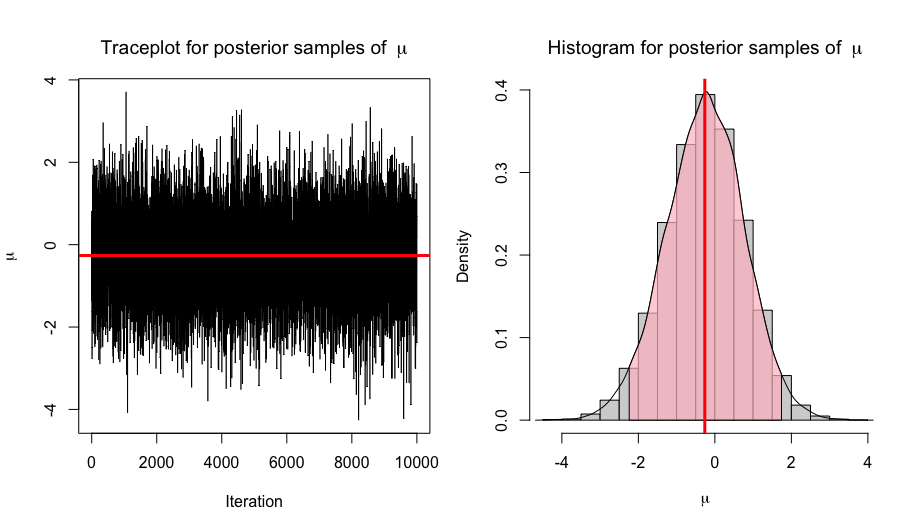
\includegraphics[scale = 0.4]{Prob3_mu.png}\\
        % 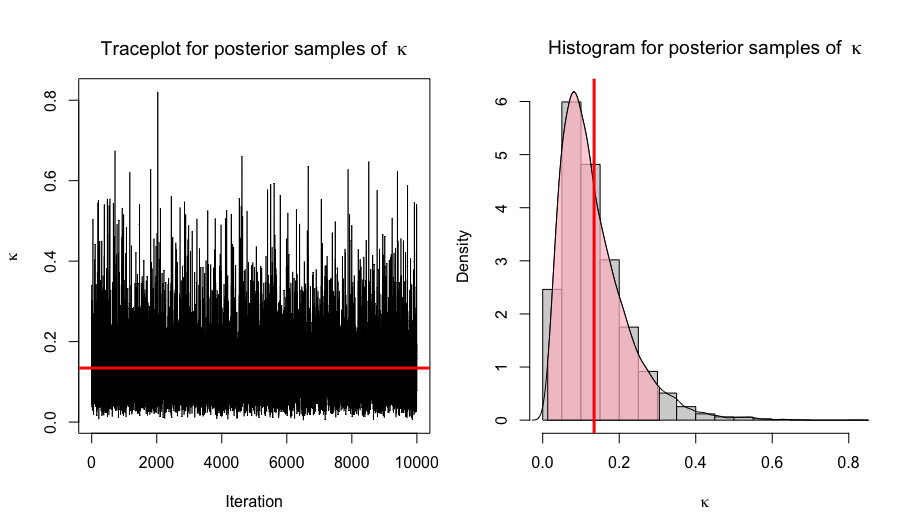
\includegraphics[scale = 0.4]{Prob3_Kappa.png}\\
        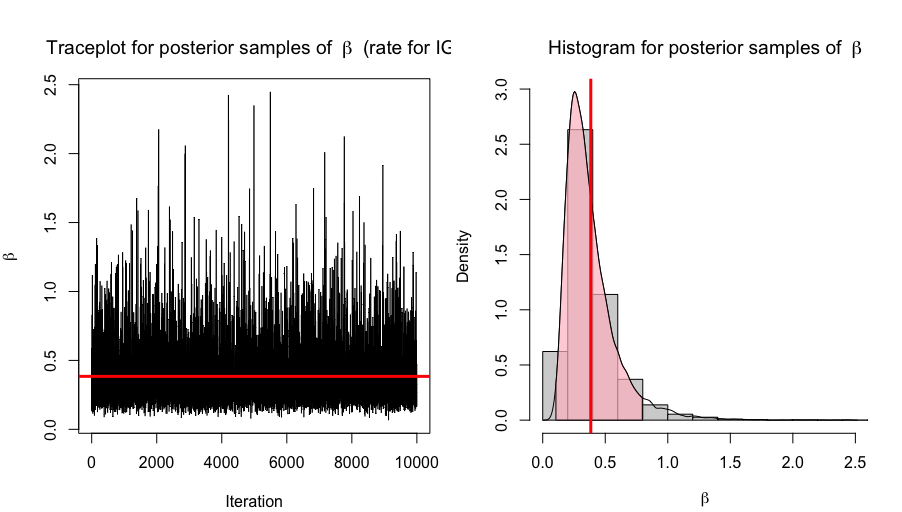
\includegraphics[scale = 0.4]{Prob3_beta.png}\\
        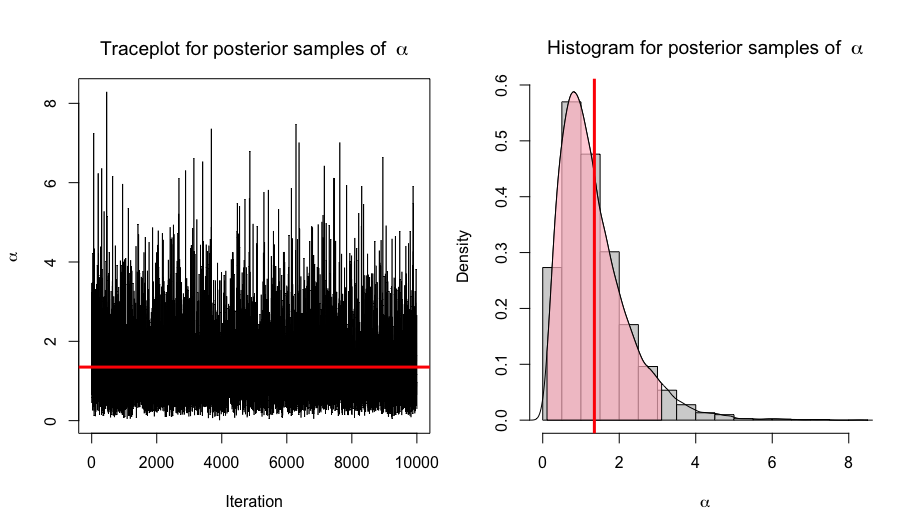
\includegraphics[scale = 0.4]{Prob3_alpha.png}\\
        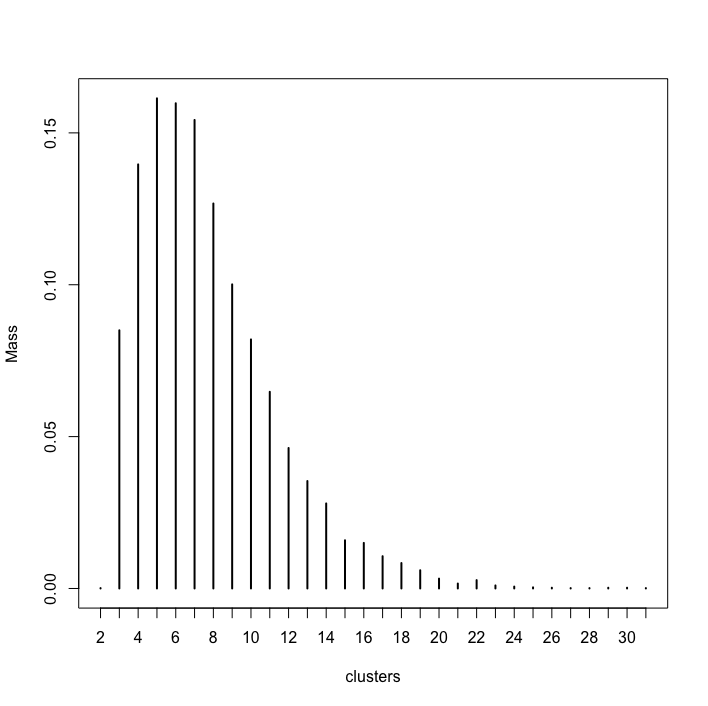
\includegraphics[scale=0.3]{Prob3_clusters.png}
        \caption{Traceplot and histogram for the posterior samples of the rate parameter for the inverse-gamma, $\beta$, (top), and $\alpha$ (middle). The posterior for the number of clusters is the bottom figure.}
        \label{prob3_fig}
    \end{figure}
    
\end{enumerate}
\end{document}